the SEG/EAGE Salt and Overthrust Modelsを用いて実験を行います.

\begin{figure}[htbp]\label{fig:true_velocity_model}
\begin{center}
    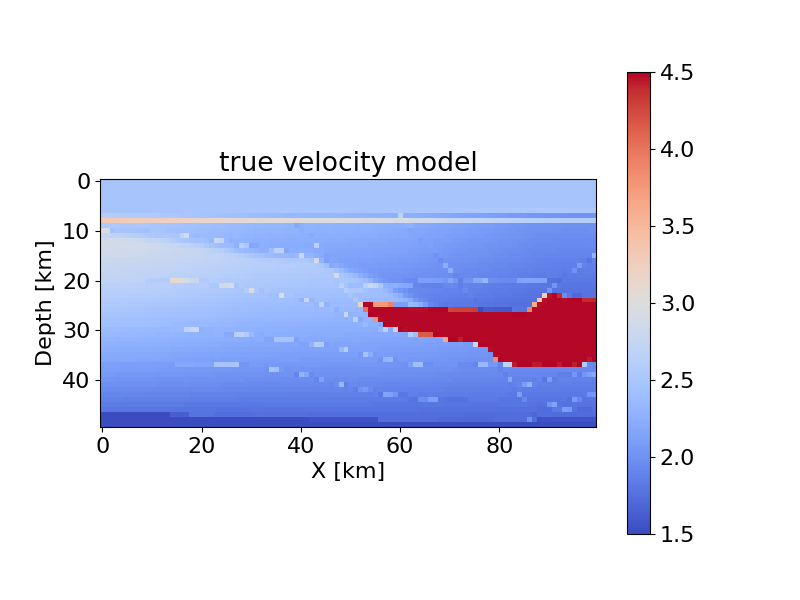
\includegraphics[width=80mm]{public/true}
    \caption{true}
\end{center}
\vspace{-\baselineskip}
\end{figure}

\begin{figure}[htbp]\label{fig:initial_velocity_model}
\vspace{-\baselineskip}
\begin{center}
    
\includegraphics[width=80mm]{public/initial}
    \caption{initial}
\end{center}
\vspace{-\baselineskip}
\end{figure}

\begin{figure}[htbp]\label{fig:gradient_velocity_model}
\vspace{-\baselineskip}
\begin{center}
    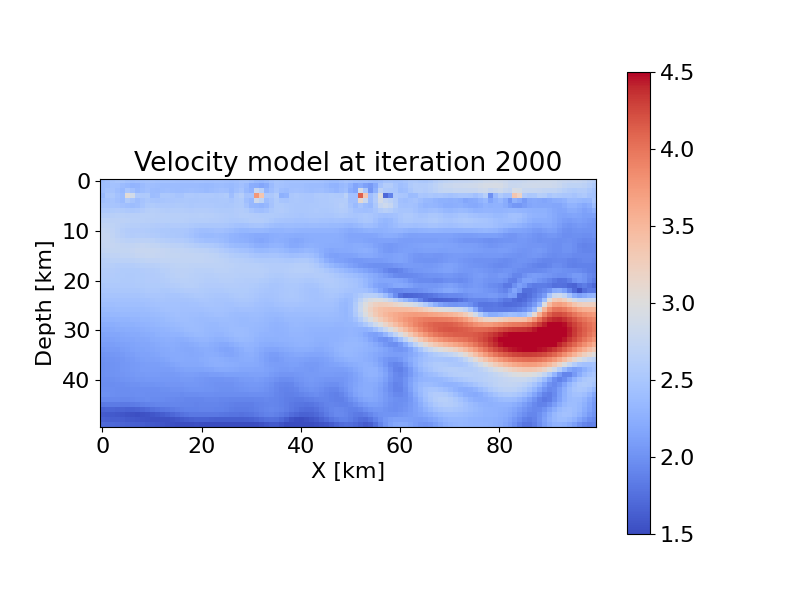
\includegraphics[width=80mm]{public/gradient}
    \caption{gradient}
\end{center}
\vspace{-\baselineskip}
\end{figure}

\begin{figure}[htbp]\label{fig:pds_velocity_model}
\vspace{-\baselineskip}
\begin{center}
    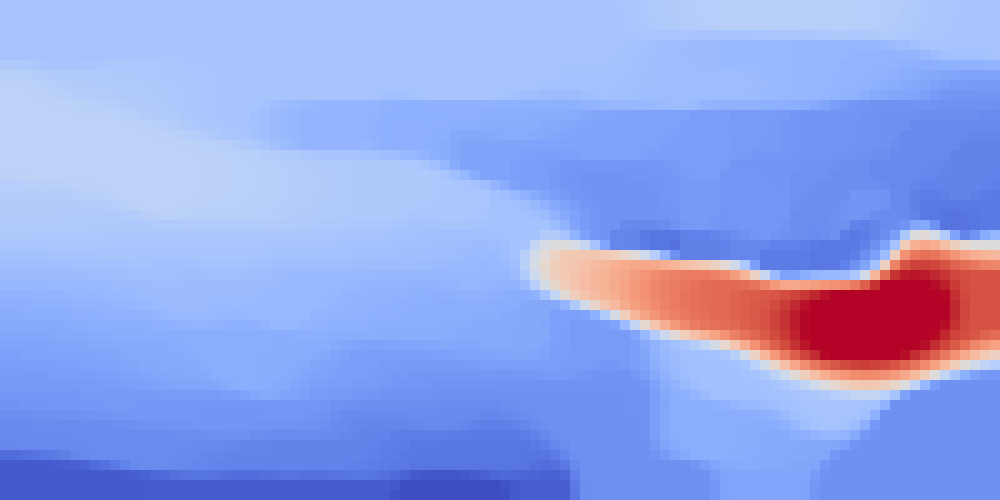
\includegraphics[width=80mm]{public/pds}
    \caption{pds}
\end{center}
\vspace{-\baselineskip}
\end{figure}

\begin{figure}[htbp]\label{fig:ssim}
\vspace{-\baselineskip}
\begin{center}
    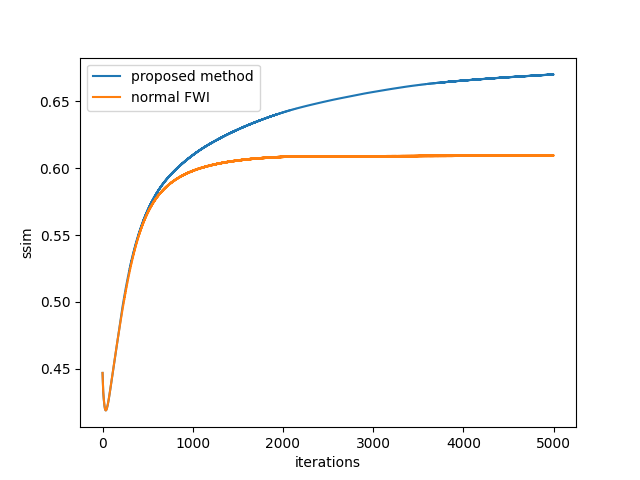
\includegraphics[width=80mm]{public/ssim}
    \caption{ssim}
\end{center}
\vspace{-\baselineskip}
\end{figure}
